%\documentclass[handout,12pt]{beamer}
\documentclass[12pt]{beamer}


%\usepackage{palatino}
%\usepackage[mathcal]{euscript}
%\usepackage[mathbf,mathcal]{euler}
\usepackage{mathbbol}
\usepackage{multicol}
\usepackage{todonotes}

%\usefonttheme{serif}
%\usefonttheme[onlymath]{serif}

%!TEX root = BanditConvex.tex

\mode<presentation>
{
  \usetheme{Madrid}
  \usecolortheme{beaver}
%  \setbeamercovered{transparent}
%  \setbeamertemplate{items}[circle]
%\setbeamertemplate{itemize items}[default]
%\setbeamertemplate{enumerate items}[default]


%\setbeamertemplate{itemize item}{\scriptsize\raise1.25pt\hbox{\donotcoloroutermaths$\blacktriangleright$}}
\setbeamertemplate{itemize subitem}{\tiny\raise1.5pt\hbox{\donotcoloroutermaths$\blacktriangleright$}}
%\setbeamertemplate{itemize subsubitem}{\tiny\raise1.5pt\hbox{\donotcoloroutermaths$*$}}
%\setbeamertemplate{enumerate item}{\insertenumlabel.}
%\setbeamertemplate{enumerate subitem}{\insertenumlabel.\insertsubenumlabel}
%\setbeamertemplate{enumerate subsubitem}{\insertenumlabel.\insertsubenumlabel.\insertsubsubenumlabel}
%\setbeamertemplate{enumerate mini template}{\insertenumlabel}
}

\definecolor{mygreen}{cmyk}{0.82,0.11,1,0.25}
\colorlet{darkgreen}{green!50!black}
\setbeamercolor{block title}{bg=mygreen,fg=white}%bg=background, fg= foreground
%\setbeamercolor{block body}{bg=yellow,fg=green}%bg=background, fg= foreground


\setbeamertemplate{blocks}[rounded][shadow=false]
\addtobeamertemplate{block begin}{\pgfsetfillopacity{0.8}}{\pgfsetfillopacity{1}}
\setbeamercolor{structure}{fg=mygreen}
%\setbeamercolor*{block title idea}{fg=blue!50,bg= blue!10}
%\setbeamercolor*{block body idea}{fg= blue,bg= blue!5}


\newenvironment<>{idea}[1]{
  \setbeamercolor{block title}{fg=white,bg=blue!75!black!80!white}
  \begin{block}#2{#1}}{\end{block}}

\newenvironment<>{brownblock}[1]{
  \setbeamercolor{block title}{fg=white,bg=yellow!50!black!80!white}
  \begin{block}#2{#1}}{\end{block}}

%\usepackage{natbib}
\setbeamertemplate{navigation symbols}{}
\setbeamertemplate{footline}[frame number]
\setbeamercolor{math text}{fg=blue!50!normal text.fg}

\usepackage{multimedia}

\makeatletter
\newcommand{\widthofbold}[1]{%
  \settowidth{\dimen0}{\textbf{#1}}%
  \makebox[\dimen0]{#1}}
\newcommand<>{\animbf}[1]{%
  \alt#2{\textbf{#1}}{\widthofbold{#1}}}
\makeatother

\usepackage{etex}
\usepackage[absolute,overlay]{textpos}

\usepackage{wasysym} % for \smiley \frownie
%
% \usepackage{wrapfig}
% \begin{wrapfigure}{POS}{WIDTH}{LINES TO RESERVE}
% ..
% \end{wrapfigure}
% The last argument is optional

% Figures need exact positioning in columns
% Use the following command to place them
\newcommand{\figincol}[1]{
\pgfputat{\pgfxy(0,0)}{\pgfbox[left,top]{#1}}
}

% ALSO:
% \pgfputat {\pgfxy(XX,YY)}{\pgfbox[left,base]{#1}}
% 
% LL = (0cm,-7cm) 
% UR = (11cm,1cm)
%
% pgfdeclareimage
% pgfuseimage

\newcommand{\Ra}{\Rightarrow}
%% BEAMER SPECIFIC COMMANDS

\newcommand{\bi}{\begin{itemize}[<+->]}
\newcommand{\ei}{\end{itemize}}
\newcommand{\bif}{\begin{itemize}}
\newcommand{\bc}{\begin{center}}
\newcommand{\ec}{\end{center}}


\setbeamercolor{math text}{fg=blue!50!normal text.fg}
\newcommand{\animframe}[2]{\begin{frame}[<+->]{#1}#2\end{frame}}
\newcommand{\animframesq}[2]{\begin{frame}[<+->][shrink,squeeze]{#1}#2\end{frame}}
\newcommand{\animframejsq}[2]{\begin{frame}[<+->][squeeze]{#1}#2\end{frame}}

\newcommand{\animframen}[2]{\begin{frame}[<+->]{#1}#2\emptynote\end{frame}}
\newcommand{\animframesqn}[2]{\begin{frame}[<+->][shrink,squeeze]{#1}#2\emptynote\end{frame}}
\newcommand{\animframejsqn}[2]{\begin{frame}[<+->][squeeze]{#1}#2\emptynote\end{frame}}

\newcommand{\myframe}[2]{\begin{frame}{#1}#2\end{frame}}
\newcommand{\myframesq}[2]{\begin{frame}[shrink,squeeze]{#1}#2\end{frame}}
\newcommand{\myframejsq}[2]{\begin{frame}[squeeze]{#1}#2\end{frame}}

\newcommand{\myframen}[2]{\begin{frame}{#1}#2\emptynote\end{frame}}
\newcommand{\myframesqn}[2]{\begin{frame}[shrink,squeeze]{#1}#2\emptynote\end{frame}}
\newcommand{\myframejsqn}[2]{\begin{frame}[squeeze]{#1}#2\emptynote\end{frame}}


%\setbeamertemplate{footline}[frame number]
\newtheorem{Solution}[theorem]{Solution}
\newtheorem{Comm}[theorem]{Comment}
\newtheorem{Note}[theorem]{Note}

\newcommand{\bcol}[1][t]{\begin{columns}[#1]} % optional argument: alignment (t,b,c)
\newcommand{\ecol}{\end{columns}}
\newcommand{\col}[1][0.5\textwidth]{\column{#1}} % argument: width of the column
%\parindent = 10pt
\newcommand{\scaletext}[3]{ % scale-factor original-width TEXT
\scalebox{#1}{\begin{minipage}[h]{#2\textwidth} #3 \end{minipage}
}}

% note: beamer slides are 128mm by 96 mm
\newcommand{\putatUL}[4]{ % width xpos ypos WHAT; upper left corner is put at the said pos
\begin{textblock*}{#1}[0,0](#2,#3)
#4
 \end{textblock*}
}
\newcommand{\putatBR}[4]{ % width xpos ypos WHAT; bottom right corner is put at the said pos
\begin{textblock*}{#1}[1,1](#2,#3)
#4
 \end{textblock*}
}
\newcommand{\putatBL}[4]{ % width xpos ypos WHAT; bottom left corner is put at the said pos
\begin{textblock*}{#1}[0,1](#2,#3)
#4
 \end{textblock*}
}
\newcommand{\putatUR}[4]{ % width xpos ypos WHAT; upper right corner is put at the said pos
\begin{textblock*}{#1}[1,0](#2,#3)
#4
 \end{textblock*}
 }
\newcommand{\putatMID}[4]{ % width xpos ypos WHAT; middle of pic is put at the said pos
\begin{textblock*}{#1}[0.5,0.5](#2,#3)
#4
 \end{textblock*}
 }
\newcommand{\putatUM}[4]{ % width xpos ypos WHAT; upper-middle of pic is put at the said pos
\begin{textblock*}{#1}[0.5,0](#2,#3)
#4
 \end{textblock*}
 }
\newcommand{\putatLM}[4]{ % width xpos ypos WHAT; lower-middle of pic is put at the said pos
\begin{textblock*}{#1}[0.5,1.0](#2,#3)
#4
 \end{textblock*}
 }

\newcommand{\putat}[3]{\begin{picture}(0,0)(0,0)\put(#1,#2){#3}\end{picture}} % xrelpos yrelpos WHAT

\makeatletter
\newcommand{\insertprevframe}[1]{
	\def\beamer@origlmargin{\Gm@lmargin}
%    \vbox{\hfill\insertslideintonotes{0.125}\hskip-\Gm@rmargin\hskip0pt%
%      \vskip-0.125\paperheight\nointerlineskip}%
	\insertslideintonotes{#1}
}

%\newcommand{\insertslideintonotes}[1]{{%
%  \begin{pgfpicture}{0cm}{0cm}{#1\paperwidth}{#1\paperheight}
%    \begin{pgflowlevelscope}{\pgftransformscale{#1}}%
%      \color[gray]{0.8}
%      \pgfpathrectangle{\pgfpointorigin}{\pgfpoint{\paperwidth}{\paperheight}}
%      \pgfusepath{fill}
%      \color{black}
%      {\pgftransformshift{\pgfpoint{\beamer@origlmargin}{\footheight}}\pgftext[left,bottom]{\copy\beamer@frameboxcopy}}
%    \end{pgflowlevelscope}
%  \end{pgfpicture}%
%  }}
\makeatother
% For adding items to the notes pages (we do not want animation there)
\newcommand{\bin}{\bi[<1->]}


\usetikzlibrary{positioning} 

\newcommand{\todoc}[2][]{\todo[color=blue!10,size=\tiny,#1]{Cs: #2}}


%!TEX root = BanditConvex.tex

\usepackage[normalem]{ulem}

%\usepackage{stmaryrd}
%\usepackage{dsfont}

%\usepackage{booktabs}
%\usepackage{multirow}
%\usepackage{colortbl}
%\usepackage{hhline}
%\usepackage{paralist}

%\usepackage{minted} % syntax highlighting
%\definecolor{mintedbg}{rgb}{0.95,0.95,0.95} %$ for bgcolor

\usepackage{pdfsync}
\usepackage{graphicx} % more modern
%\usepackage{epsfig} % less modern

% Hyperlinks make it very easy to navigate an electronic document.
% In addition, this is where you should specify the thesis title
% and author as they appear in the properties of the PDF document.
% Use the "hyperref" package
% N.B. HYPERREF MUST BE THE SECOND TO LAST PACKAGE LOADED; ADD ADDITIONAL PKGS ABOVE
%\usepackage[pdftex,letterpaper=true,pagebackref=false]{hyperref} % with basic options
		% N.B. pagebackref=true provides links back from the References to the body text. This can cause trouble for printing.
\hypersetup{
    plainpages=false,       % needed if Roman numbers in frontpages
    pdfpagelabels=true,     % adds page number as label in Acrobat's page count
    bookmarks=true,         % show bookmarks bar?
    unicode=false,          % non-Latin characters in Acrobat’s bookmarks
    pdftoolbar=true,        % show Acrobat’s toolbar?
    pdfmenubar=true,        % show Acrobat’s menu?
    pdffitwindow=false,     % window fit to page when opened
    pdfstartview={FitH},    % fits the width of the page to the window
    pdftitle={(Bandit) Convex Optimization with Biased Noisy Gradient Oracles},    % set
    pdfauthor={},    % set
%     pdfauthor={D\'avid Szepesv\'ari},    % set
%    pdfsubject={Subject},  % subject: CHANGE THIS TEXT! and uncomment this line
%    pdfkeywords={keyword1} {key2} {key3}, % list of keywords, and uncomment this line if desired
    pdfnewwindow=true,      % links in new window
    colorlinks=true,        % false: boxed links; true: colored links
    linkcolor=blue,         % color of internal links
    citecolor=blue,        % color of links to bibliography
    filecolor=magenta,      % color of file links
    urlcolor=cyan           % color of external links
}


%\newcommand{\todog}{\todo[color=green]}

%\usepackage[disable]{todonotes}
\usepackage{todonotes}
% todo by Csaba
%\newcommand{\todoc}[2][]{\todo[color=blue!20!white,#1]{Csaba: #2}}
% todo by Yasin
\newcommand{\todoy}[2][]{\todo[color=red!20!white,#1]{Yasin: #2}}
% todo by David
\newcommand{\todod}[2][]{\todo[color=green!20!white,#1]{Yasin: #2}}



% For citations
%\usepackage[round,sectionbib]{natbib}
% See:
% http://merkel.zoneo.net/Latex/natbib.php
%\bibpunct{[}{]}{;}{n}{}{,}

\usepackage{algorithm}
\usepackage{algpseudocode}
%\usepackage{algorithmic}

\usepackage{amssymb}
%\usepackage[dvips]{graphics}

\usepackage{amsmath} % Learn about the AMS package, again very useful!
\usepackage{amsthm}
\usepackage{mathtools} % MoveEqLeft
\usepackage{color}
\usepackage{graphicx}
\usepackage{epstopdf}
%\usepackage{stmaryrd}
%\usepackage{algorithm,algorithmic}
\usepackage{verbatim} 

%\usepackage{mathabx}

\usepackage{nicefrac}

\usepackage{enumerate}
%\usepackage{dsfont}
%\usepackage{subfig}
%\usepackage{small-headings}

%\usepackage{cleveref}

% this is not needed at the end..
% \usepackage{etoolbox} \ifstrempty{STR}{IF EMPTY}{IF NOT EMPTY}

% Turn on/off notes and descriptions of research problems
\newif\ifcomm
%\commfalse % also turns off internal todo comments
\commtrue

\newif\iflong
\longtrue
%\longfalse


% THEOREMS -------------------------------------------------------
\newtheorem{thm}{Theorem}%[chapter]
\newtheorem{cor}[thm]{Corollary}
\newtheorem{lem}[thm]{Lemma}
\newtheorem{prop}[thm]{Proposition}
\newtheorem{conj}[thm]{Conjecture}
\newtheorem{defn}[thm]{Definition}
\newtheorem{rem}[thm]{Remark}

%\newtheorem{name}{Printed output}[numberby]

%\newtheorem{lemma}{Lemma}
%\newtheorem{definition}[lemma]{Definition}
%\newtheorem{theorem}[lemma]{Theorem}
%\newtheorem{proposition}[lemma]{Proposition}
%\newtheorem{corollary}[lemma]{Corollary}

\DeclareMathOperator{\Exp}{\mathbf{E}}
\newcommand{\V}{\overline{V}}
\newcommand{\X}{\mathbf{X}}
\newcommand{\Y}{\mathbf{Y}}
\newcommand{\ETA}{\mathbf{\eta}}
\newcommand{\bPhi}{\mathbf{\Phi}}

%\renewtheorem{definition}[thm]{Definition}
%\theoremstyle{definition}
%\newtheorem{remark}[thm]{Remark}

\newcounter{assumption}%[section]
\renewcommand{\theassumption}{A\arabic{assumption}}
\newenvironment{ass}[1][]{\begin{trivlist}\item[] \refstepcounter{assumption}%
 {\bf Assumption\ \theassumption\ #1} }{%\par\nobreak\noindent\sl\ignorespaces}{%
 \ifvmode\smallskip\fi\end{trivlist}}

\def\ddefloop#1{\ifx\ddefloop#1\else\ddef{#1}\expandafter\ddefloop\fi}

% \bA, \bB, ...
\def\ddef#1{\expandafter\def\csname b#1\endcsname{\ensuremath{\mathbf{#1}}}}
\ddefloop ABCDEFGHIJKLMNOPQRSTUVWXYZ\ddefloop

% \bbA, \bbB, ...
\def\ddef#1{\expandafter\def\csname bb#1\endcsname{\ensuremath{\mathbb{#1}}}}
\ddefloop ABCDEFGHIJKLMNOPQRSTUVWXYZ\ddefloop

% \cA, \cB, ...
\def\ddef#1{\expandafter\def\csname c#1\endcsname{\ensuremath{\mathcal{#1}}}}
\ddefloop ABCDEFGHIJKLMNOPQRSTUVWXYZ\ddefloop

% \vecA, \vecB, ..., \veca, \vecb, ...
\def\ddef#1{\expandafter\def\csname vec#1\endcsname{\ensuremath{\boldsymbol{#1}}}}
\ddefloop ABCDEFGHIJKLMNOPQRSTUVWXYZabcdefghijklmnopqrstuvwxyz\ddefloop

% \valpha, \vbeta, ...,  \vGamma, \vDelta, ...,
\def\ddef#1{\expandafter\def\csname v#1\endcsname{\ensuremath{\boldsymbol{\csname #1\endcsname}}}}
\ddefloop {alpha}{beta}{gamma}{delta}{epsilon}{varepsilon}{zeta}{eta}{theta}{vartheta}{iota}{kappa}{lambda}{mu}{nu}{xi}{pi}{varpi}{rho}{varrho}{sigma}{varsigma}{tau}{upsilon}{phi}{varphi}{chi}{psi}{omega}{Gamma}{Delta}{Theta}{Lambda}{Xi}{Pi}{Sigma}{varSigma}{Upsilon}{Phi}{Psi}{Omega}\ddefloop

\newcommand\Sig{\ensuremath{\varSigma}}
\newcommand\veps{\ensuremath{\varepsilon}}
\newcommand\eps{\ensuremath{\epsilon}}

\renewcommand\t{{\ensuremath{\scriptscriptstyle{\top}}}}

%\newenvironment{remark}

%\newenvironment{proof}{{\bf Proof.}}{\hfill\rule{2mm}{2mm}\\}

% Keep whatever you need from here

\newcommand{\bd}[1]{\mathbf{#1}}

\newcommand{\norm}[1]{\left\Vert#1\right\Vert}
\newcommand{\smallnorm}[1]{\|#1\|}
\newcommand{\abs}[1]{\left\vert#1\right\vert}
\newcommand{\supnorm}[1]{\norm{#1}_\infty}
\newcommand{\trace}{\mathop{\rm trace}}
\newcommand{\maxEig}{\lambda_{\mbox{max}}}

%\newcommand{\set}[1]{\left\{#1\right\}}
\newcommand{\cset}[2]{\left\{\,#1\,:\,#2\,\right\}}

\renewcommand{\natural}{\mathbb N}                   % Natural numbers
\newcommand{\Real}{\mathbb R}                        % Real numbers
\newcommand{\real}{\mathbb R}                        % again..
\newcommand{\R}{{\mathbb{R}}}                        % again..

\newcommand{\vv}{\vspace*{-2mm}}
\newcommand{\hh}{\hspace*{4mm}}
\newcommand{\hfig}{\hrule\vspace*{-5mm}}


\newcommand{\Prob}[1]{{\mathbb P}\left(#1\right)}    % Probabilities; example: \Prob{X>\eps}<1-\delta
\renewcommand{\P}{{\mathbb P}}                         % Probabilities when we want to control the parenthesis
\newcommand{\EE}[1]{{\mathbb E}\left[#1\right]}      % Expectations
\newcommand{\E}{{\mathbb E}}                         % Expectations  when we want to control the parenthesis
\newcommand{\Var}[1]{{\mathrm{Var}}\left[#1\right]}  % Variances
%\newcommand{\one}{\mathbb I}
\newcommand{\one}[1]{{\mathbb I}_{\{#1\}}}           % Characteristic function

\newcommand{\MB}{\mathcal{B}}
\newcommand{\MA}{\mathcal{A}}
\newcommand{\MS}{\mathcal{S}}
\newcommand{\MF}{\mathcal{F}}
\newcommand{\MG}{\mathcal{G}}
\newcommand{\MH}{\mathcal{H}}
\newcommand{\MC}{\mathcal{C}}
\newcommand{\MRR}{\mathcal{R}}
\newcommand{\MD}{\mathcal{D}}
\newcommand{\MP}{\mathcal{P}}
\newcommand{\MU}{\mathcal{U}}
\newcommand{\MO}{\mathcal{O}}
\newcommand{\MX}{\mathcal{X}}
\newcommand{\MZ}{\mathcal{Z}}
\newcommand{\MN}{\mathcal{N}}
\newcommand{\MM}{\mathcal{M}}
\newcommand{\MR}{\mathcal{R}}
\newcommand{\ME}{\mathcal{E}}
\newcommand{\MT}{\mathcal{T}}

\newcommand{\GG}{\mathcal{G}}


%\newcommand{\eps}{\varepsilon}                       % Nice epsilon
\newcommand{\ep}{\varepsilon}                        % Shorthand for nice epsilon
\newcommand{\de}{\delta}                             % Shorthand for delta
\newcommand{\To}{\longrightarrow}
\newcommand{\ra}{\rightarrow}

\newcommand{\argmin}{\mathop{\rm argmin}}
\newcommand{\argmax}{\mathop{\rm argmax}}
\newcommand{\diag}{\mathop{\rm diag}}
\newcommand{\inlinemin}{\wedge}
\newcommand{\inlinemax}{\vee}

\newcommand{\ip}[1]{\langle #1\rangle}
\newcommand{\eqdef}{\doteq} %\stackrel{\mbox{\rm\tiny def}}{=}}
\newcommand{\aP}{{\cal P}}

% Shorthands I use for math environments
\newcommand{\beq}{\begin{equation}}
\newcommand{\eeq}{\end{equation}}
\newcommand{\beqa}{\begin{eqnarray}}
\newcommand{\eeqa}{\end{eqnarray}}
\newcommand{\beqan}{\begin{eqnarray*}}
\newcommand{\eeqan}{\end{eqnarray*}}
\newcommand{\ben}{\begin{eqnarray*}}
\newcommand{\een}{\end{eqnarray*}}
\newcommand{\bea}{\begin{align*}}
\newcommand{\eea}{\end{align*}}


\newcommand{\RA}{$\Rightarrow$}
\ifcomm
   \newcommand\comm[1]{\textcolor{blue}{ #1}}
   \newcommand{\mtodo}[2]{\todo{{\bf #1}: #2}} % To add comments into the text; the first argument is "who", the second is "what"
   \def\here#1{{\bf $\langle\langle$#1$\rangle\rangle$}}

\else
   \newcommand\comm[1]{}
   \newcommand{\mtodo}[2]{}
   \def\here#1{}
\fi
\newcommand{\remove}[1]{\textcolor{blue}{\sout{#1}}}
\newcommand{\tO}{\tilde{O}}

\newcommand{\sfrac}{\nicefrac}
\newcommand{\pai}{{(i)}}
\newcommand{\integer}{\mathbb{Z}}
\renewcommand{\phi}{\varphi}
\newcommand{\ewithin}{\eps_{\text{W}}}
\newcommand{\ebetween}{\eps_{\text{B}}}
\newcommand{\emean}{\eps_{\text{M}}}
%\DeclareMathOperator{\trace}{trace}
\newcommand{\e}{\mathbf{e}}
\renewcommand{\eps}{\varepsilon}
\newcommand{\tM}{\tilde{M}}
\newcommand{\MRP}{{\cal M}}
\newcommand{\kfun}{\mathbb{K}}

\newcommand{\aparam}{\omega}
\newcommand{\dimaction}{d_{\Actions}}
\newcommand{\dimaparam}{d_{\aparam}}
\newcommand{\traj}{\xi}
\newcommand{\Trajset}{\Xi}
\newcommand{\Traj}{X}
\newcommand{\perf}{\rho}
\newcommand{\dstat}{\mu} % stationary distribution underlying a Markov chain
\newcommand{\Regret}{{\bf R}}
\renewcommand{\AA}{{\cal A}}
%\newcommand{\SA}{\States\times\Actions}
\newcommand{\Sample}{{\cal D}}
\newcommand{\hA}{\hat{A}}
\newcommand{\hb}{\hat{b}}
\newcommand{\ZZ}{{\cal Z}}
\newcommand{\ttop}{^\top}
\newcommand{\Stexpra}{\sum_{k=1}^{t} \eta_k m_{k-1}}
\newcommand{\Stexpraz}{\sum_{k=1}^{t} \eta_k z_{k-1}}
\newcommand{\Vinit}{V}
\newcommand{\Us}{U_s}
\newcommand{\Vtexpra}{\Vinit +\sum_{k=1}^t m_{k-1} m_{k-1}\ttop }
\newcommand{\CPE}[2]{\EE{ #1 \,| #2 }}
\newcommand{\PP}[1]{\mathbb{P}\left( #1\right)}
\newcommand{\normm}[2]{\norm{#1}_{#2}}
\newcommand{\Vta}[1]{\overline{V}_{#1}}
\newcommand{\Vt}{\Vta{t}}
\newcommand{\Vtta}[1]{V_{#1}}
\newcommand{\Vtt}{\Vtta{t}}
\newcommand{\beps}{\mathbb{\varepsilon}}
\newcommand{\bw}{\mathbf{w}}

\newcommand{\FF}{{\cal F}}
\newcommand{\CrossRef}[1]{#1}

\newcommand{\oZ}{\overline{Z}}
\newcommand{\oA}{\overline{A}}
\newcommand{\eqf}[1]{\exp({#1})-1-#1}
\newcommand{\orho}{\overline{\rho}}
\newcommand{\QQ}{{\cal Q}}

\newcommand{\mfrac}[2]{{}^{#1}/_{#2}}


\newcommand{\hth}{\widehat{\theta}}
\newcommand{\tth}{\widetilde{\theta}}
\newcommand{\hTh}{\widehat\Theta}
\newcommand{\TTh}{\widetilde\Theta}
\newcommand{\Xmax}{X_{\max}}
\newcommand{\Zmax}{Z_{\max}}
\newcommand{\bVparam}[1]{\mathbf{V}_{#1}}
\newcommand{\bVn}{\bVparam{n}}
\newcommand{\bVt}{\bVparam{t}}
\newcommand{\BVt}{\overline{\bV}_{t}}
\newcommand{\BVta}{\overline{\bV}_{\tau}}

% for Hilbert spaces
\newcommand{\keybound}[3]{
2 R^2 \log\left( \frac{\det\left(I + #2_{1:#3}#1^{-1}#2_{1:#3}^*\right)^{\sfrac12}}{\delta} \right)
%2 R^2 \log\left( \frac{\det (\Vta{\tau})^{\nicefrac12}\det(\Us)^{-\nicefrac{\kern-2pt-\kern-2pt 1}{2}}}{\delta} \right)
}
\newcommand{\keyboundappliedp}[2]{
 R \sqrt{2 \log\left( \frac{\det (I + #2_{1:#1}#2_{1:#1}^*/\lambda)^{\sfrac12}}{\delta} \right)}
}
\newcommand{\keyboundapplied}[1]{\keyboundappliedp{t}{#1}}
\newcommand{\keyboundappliedworstp}[1]{
 R \sqrt{\frac{#1 L^2}{\lambda} + 2\log\left( \frac{1}{\delta}\right) }
}
\newcommand{\keyboundappliedworst}{\keyboundappliedworstp{t}}

% for Euclidean spaces
\newcommand{\keyboundEuclidean}[1]{
2 R^2 \log\left( \frac{\det (\Vta{#1})^{\nicefrac12}\det(\Vinit)^{\nicefrac{\kern-2pt-\kern-2pt 1}{2}}}{\delta} \right)
}

\newcommand{\keyboundappliedpEuclidean}[1]{
 R \sqrt{2 \log\left( \frac{\det (\V_{#1})^{1/2}\det(\lambda I)^{-1/2}}{\delta} \right)}
}
\newcommand{\keyboundappliedEuclidean}{\keyboundappliedpEuclidean{t}}
\newcommand{\keyboundappliedworstpEuclidean}[1]{
 R \sqrt{d \log\left( \frac{1+\frac{#1 L}{\lambda}}{\delta} \right)}
}
\newcommand{\keyboundappliedworstEuclidean}{\keyboundappliedworstpEuclidean{t}}

% for LQR
\newcommand{\keyboundappliedplqr}[1]{
 n L \sqrt{2 \log\left( \frac{\det (\V_{#1})^{\sfrac12}\det(\lambda I)^{\sfrac{\kern-2pt-\kern-2pt 1}{2}}}{\delta} \right)}
}
\newcommand{\keyboundappliedlqr}{\keyboundappliedplqr{t}}
 \newcommand{\keyboundappliedlqrworstp}[1]{
 n L \sqrt{(n+d) \log\left( \frac{1+\frac{#1 c_m}{\lambda}}{\delta} \right)}
}
 \newcommand{\keyboundappliedlqrworst}{\keyboundappliedlqrworstp{t}}


\newcommand{\DR}{D_{\mathcal{R}}}


\title{(Bandit) Convex Optimization with\\
 Biased Noisy Gradient Oracles}
\institute{
Reinforcement Learning and Artificial Intelligence (RLAI) Group\\
 Department of Computing Science \& AICML\\ 
 University of Alberta \\ 
 \href{mailto:csaba.szepesvari@ualberta.ca}{\texttt{csaba.szepesvari@ualberta.ca}}
% \href{mailto:jneufeld@ualberta.ca}{\texttt{jneufeld@ualberta.ca}}
\\ 
\vspace{0.5cm}
%\includegraphics[scale=0.9]{google-logo} 
%\hspace{2cm} \vspace{0.5cm} 

\includegraphics[scale=0.3]{figs/u-of-alberta-logo}
 }
%\author{James Neufeld}
\author{Csaba Szepesv\'ari}
%\date{February 13, 2014}
%\date{May 23, 2014}
%\date{June 7, 2014}
%\date{June 22, 2014}
%\date{April 2, 2015}
\date{November 10, 2015}

\usepackage{natbib}
%\bibliographystyle{apalike}
\bibliographystyle{apalike}
%\bibliographystyle{alpha}

\DeclareMathOperator{\supp}{supp}
% number sets
\newcommand{\N}{{\mathbb N}}
%\newcommand{\R}{{\mathbb R}}
%\newcommand{\real}{{\mathbb R}}

% spaces, vectors, matrices, distributions
%\newcommand{\eps}{\varepsilon}
\renewcommand{\H}{{\mathcal H}}
%\newcommand{\X}{\mathbf{X}}
%\newcommand{\Y}{\mathbf{Y}}
%\newcommand{\E}{{\mathcal E}}
\newcommand{\F}{{\mathcal F}}
\newcommand{\G}{{\mathcal G}}
\newcommand{\Z}{{\mathcal Z}}
\newcommand{\w}{{\mathbf w}}
\newcommand{\x}{{\mathbf x}}
\newcommand{\z}{{\mathbf z}}
\newcommand{\h}{{\mathbf h}}
\renewcommand{\P}{{\mathbf P}}
\renewcommand{\c}{{\mathbf c}}
\newcommand{\M}{{\mathbf M}}
\newcommand{\y}{{\mathbf y}}
\newcommand{\D}{{\mathcal D}}
%\newcommand*{\newblock}{}
%\newcommand{\ip}[1]{\langle #1\rangle}
%\newcommand{\norm}[1]{\left\|#1\right\|}
\newcommand{\tnorm}[1]{\|#1\|}
\newcommand{\A}{\mathcal{A}}
%\newcommand{\one}[1]{\mathbb{I}_{\{#1\}}}
%\newcommand{\EE}[1]{\mathbb{E}[#1]}
%\newcommand{\EEgrow}[1]{\mathbb{E}\left[#1\right]}

% operators
%\DeclareMathOperator*{\Exp}{\mathbf{E}}   % expectation
%\DeclareMathOperator*{\Prob}{\mathbf{Pr}}   % expectation
%\DeclareMathOperator*{\Var}{\mathbf{Var}}   % expectation
\DeclareMathOperator*{\Err}{Err}   
%\DeclareMathOperator*{\argmin}{argmin}   
\DeclareMathOperator*{\VC}{VC-dim}   
\DeclareMathOperator*{\Ldim}{L-dim}   
\DeclareMathOperator{\Rademacher}{\mathcal{R}}   
\DeclareMathOperator{\SRademacher}{\mathcal{SR}}   
\DeclareMathOperator*{\sign}{sign}   
\DeclareMathOperator*{\indicator}{\mathbb{1}}   
\DeclareMathOperator*{\minimize}{minimize}   
\DeclareMathOperator*{\conv}{conv}   
%\DeclareMathOperator{\Regret}{Regret}   
\DeclareMathOperator{\rowspace}{rowspace}   
%\DeclareMathOperator*{\argmax}{argmax}   
\DeclareMathOperator*{\polylog}{polylog}

\DeclareMathOperator*{\rows}{\#rows}   
\DeclareMathOperator*{\shattered}{\#shattered}   

\newtheorem{conjecture}{Conjecture}

\begin{document}

%%%%%%%%%%%%%%%%%%%%%%%%%%%%%%%%%%%%%%%%%%%%%%%%%%%%%%%%%%%%%%%

\begin{frame}
	\maketitle
	\vspace*{-0.4in}
	\begin{center}
          Gatsby Seminar 
	\end{center}
\end{frame}
%%%%%%%%%%%%%%%%%%%%%%%%%%%%%%%%%%%%%%%%%%%%%%%%%%%%%%%%%%%%%%%


\begin{frame}
\frametitle{Summary}

\uncover<+->{
    Questions to be answered:}
    \bi
    \item \alert{Why} should we care? 
    \item \alert{What} are the unique challenges? 
    \item \alert{How} do we address them?
    \ei
    \bigskip
    
\end{frame}

%%%%%%%%%%%%%%%%%%%%%%%%%%%%%%%%%%%%%%%%%%%%%%%%%%%%%%%%%%%%%%%

%\section{Introduction}
\begin{frame}{Outline}
\tableofcontents %[currentsection]
\end{frame}


%%%%%%%%%%%%%%%%%%%%%%%%%%%%%%%%%%%%%%%%%%%%%%%%
\section{Bandit Problems}
%%%%%%%%%%%%%%%%%%%%%%%%%%%%%%%%%%%%%%%%%%%%%%%%

% Bandit problems:
% Get value of an option
% 
% Robbins
% Bandit linear optimization
% Bandit nonlinear optimization
% Bandit convex optimization

\frame{
	\frametitle{Convex Optimization with Noisy Bandit Feedback}
	\bcol[c]
	\col
	\bc
	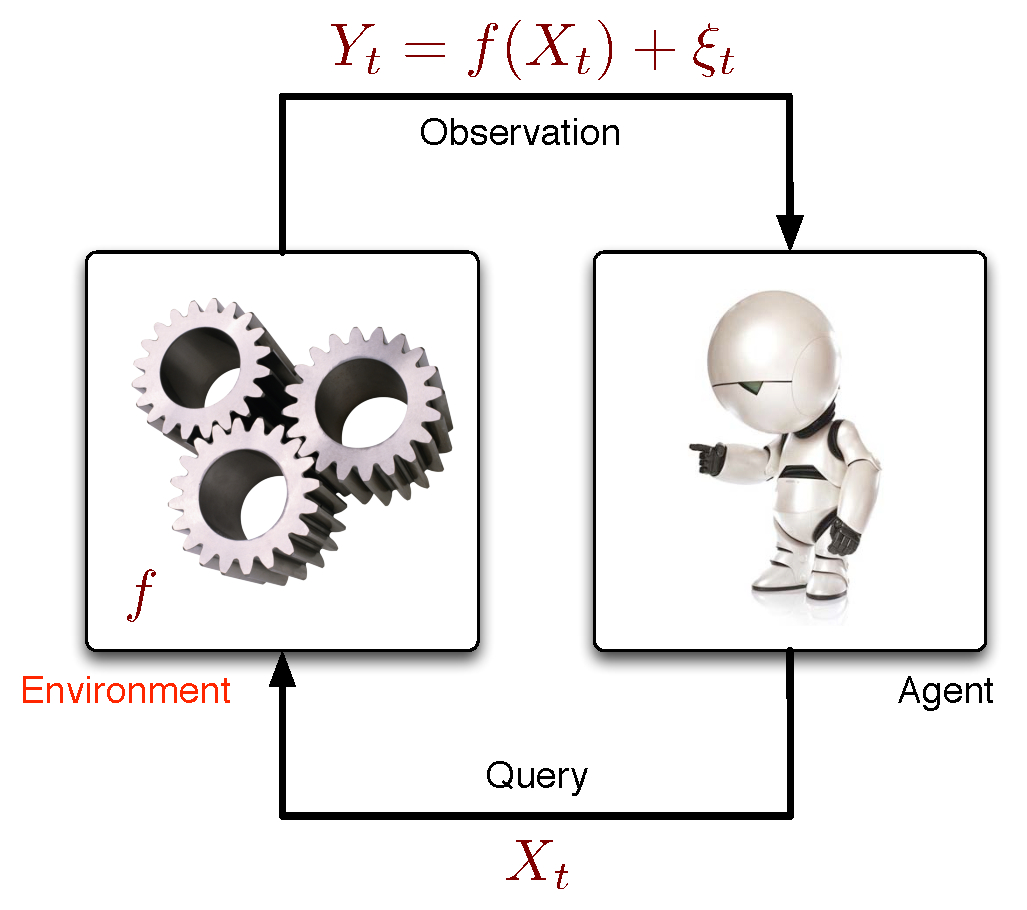
\includegraphics[width=\textwidth]{figs/Interaction}
	\ec
	\col
%	\begin{block}<+->{Goal}
	\alert{Goal}\\
	Assume $f$ convex (smooth etc).\\
	Find a near-minimizer of $f$ using $n>0$ queries!
%	\end{block}
	\bigskip
	
	\uncover<+->{
		Noisy Bandit Feedback $\equiv$ Noisy zeroth-order information\\
	}

	\ecol
	\bigskip
%	Why ``bandit''? ``Bandit theory'' \\
	% Why bandit?
	\begin{block}<+->{Main Question}
		How fast can the optimization error
		$
		\Delta_n = \EE{f(X_n) }- \inf_{x\in \cK} f(x)
		$
		 decrease with $n$?
	\end{block}
}
%%%%%%%%%%%%%%%%%%%%%%%%%%%%%%%%%%%%%%%%%%%%%%%%
\frame{
	\frametitle{Example: Resource Allocation}
	\bcol[c]
	\col[0.45\textwidth]
	\bc
	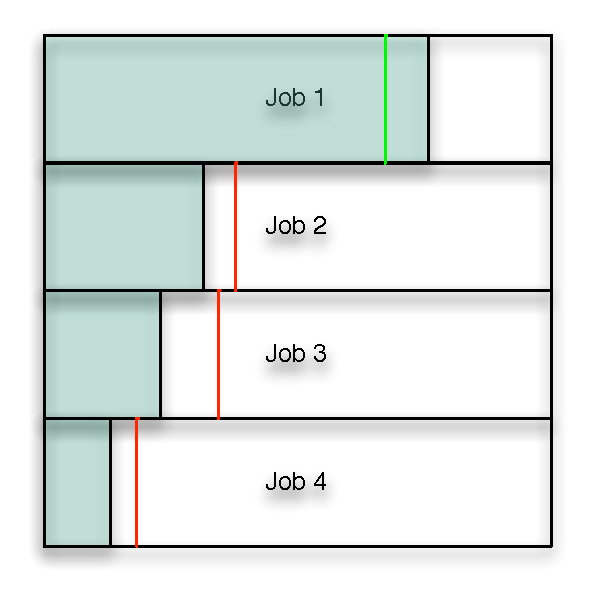
\includegraphics[width=\textwidth]{figs/memory}
	\ec
	\col[0.55\textwidth]
	\bi
	\item Distribute memory in between jobs
	\item Maximize success: $\max_x f(x)$
	\item Linear constraints: $\sum_i x_i = 1$
	\item Concave objective: Convex combination of resources not worse than what randomization gives.
	\ei
	\ecol
}

%%%%%%%%%%%%%%%%%%%%%%%%%%%%%%%%%%%%%%%%%%%%%%%%

\frame{
	\frametitle{Why Bandit Feedback?}
	\bi
	\item No other choice
		\bi
		\item Controlling an unknown system
		\item Simulation optimization: 
			\bi
			\item
				$f(x) = \EE{ F(x,\xi) }$ --- $\xi$: simulation noise
			\item $F(x,\xi)$ is the output of a simulation;
			\item Gradients are unavailable
			\ei
		\ei
	\ei
	\bigskip
	\bi
	\item By choice: 
		\bi
		\item Gradient is too expensive/complicated to compute
		\item ((Can this be justified?))
		\ei
	\ei
}

%%%%%%%%%%%%%%%%%%%%%%%%%%%%%%%%%%%%%%%%%%%%%%%%
\frame{
	\frametitle{Subclasses of Convex Problems}
	\bcol[c]
	\col
	\bc
	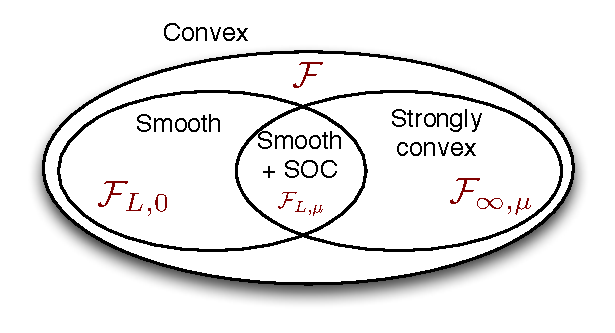
\includegraphics[width=\textwidth]{figs/Problems}
	\ec
	\col
	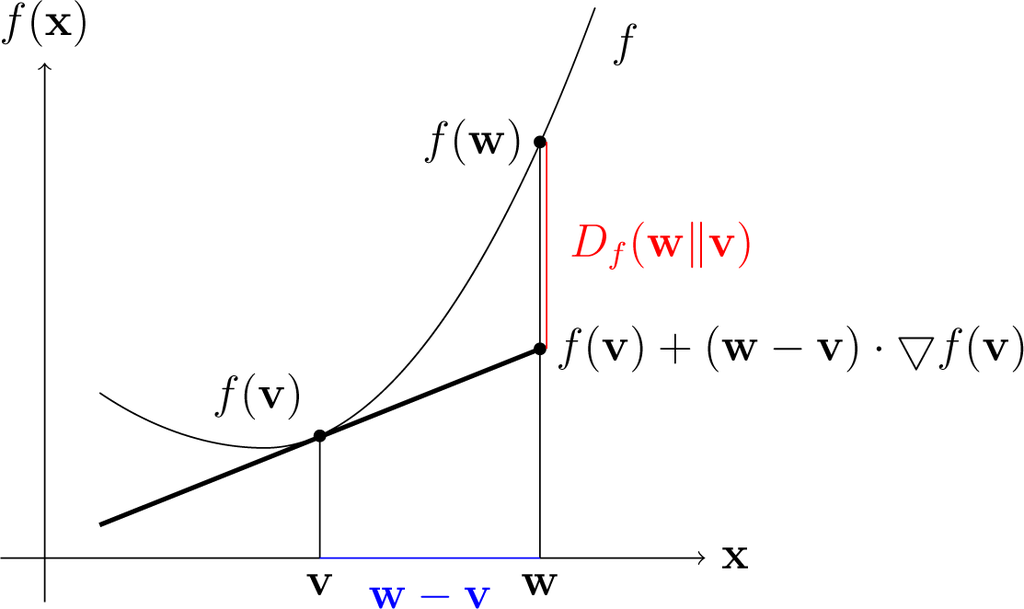
\includegraphics[width=\textwidth]{figs/entropy-16-06338f2-1024}
	\ecol
	\bi
	\item Curviness (deviation from linearity): 
	\begin{align*}
	D_f(x,y)\doteq f(x)- \left\{ f(y) + \ip{\nabla f(y),x-y} \right\}.
	\end{align*}
	\ei
	\bcol[c]
	\col[0.7\textwidth]
	\bi
	\item
	Smoothness: 
	$\qquad
	D_f(x,y) \le \frac{L}{2} \norm{x-y}^2\,.
	$
	\item
	Strong convexity:
	$
	D_f(x,y) \ge \frac{\mu}{2} \norm{x-y}^2\,.
	$
	\ei
	\col[0.3\textwidth]
	\begin{block}{}
		$\cK \subset \R^d$ convex, closed, non-empty.
	\end{block}
	\ecol

}

%%%%%%%%%%%%%%%%%%%%%%%%%%%%%%%%%%%%%%%%%%%%%%%%
\frame{
	\frametitle{Convex Optimization 101: Ellipsoid Method}
	\begin{block}{Assumption} First-order information,
	$(\nabla f(\cdot), f(\cdot))$, can be obtained at any point.
	\end{block}
	
	\bcol[b]
	\col[0.65\textwidth]
	\begin{block}{Ellipsoid Method \citep{Shor70}}
	\bi
	\item
	$\Delta_n^{\mathcal{E},d} = C\exp(-\frac{n}{d^2})$ {\footnotesize \citep{NeYu83}}	
	\item
	Matching lower bound when $d$ small and $n$ large.\\
	\uncover<+->{$\ldots$ but}
			\item Each update takes $O(d^2)$ MADDs (prohibitive when $d$ large).
			\item Suboptimal for $d/n^2 \gg 1$:
			 $\lim_{d\to\infty} \Delta_n^{\mathcal{E},d} = \Omega(1)$, while
			  $\Delta_n^* = \Theta(1/\sqrt{n})$.
	\ei
	\end{block}
	\col[0.35\textwidth]
	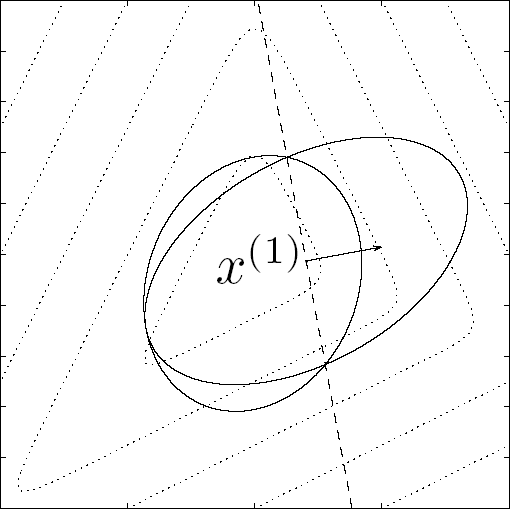
\includegraphics[width=\textwidth]{figs/Ellipsoid_2}
	\ecol
}

%%%%%%%%%%%%%%%%%%%%%%%%%%%%%%%%%%%%%%%%%%%%%%%%
\frame{
	\frametitle{Convex Optimization 101: Gradient Methods}
	Think: ``$d$ large''. Update complexity is $O(d)$.
	\bi
	\item Subgradient method: Optimal for convex problems:
	 \[\Delta_n = O(\sqrt{1/n}).\]
	\centering No dependence on $d$!
	\bigskip
	\item Gradient method + momentum term $\equiv$\\
	$\qquad$ accelerated gradient method
	\citep{nesterov2004introductory}.
	\todoc[inline]{Requires knowledge of $L$, $\mu$?}
	\bi
	\item Optimal for smooth convex problems: 
	\[ \Delta_n = O(L/n^2).	\]
	\item Optimal for strongly convex, smooth problems:
	\[ \Delta_n = \exp(- \tfrac{n}{ \sqrt{L/\mu} } ). \]
	\ei
	\ei
}

%%%%%%%%%%%%%%%%%%%%%%%%%%%%%%%%%%%%%%%%%%%%%%%%
\frame{
	\frametitle{Noisy Bandit Feedback}
	Recall: $f(x) = \EE{ F(x,\xi) }$.

	\bigskip
	\bigskip

	\begin{block}{Assumptions}
	\medskip
	\bcol
	\col[0.015\textwidth]
	\mbox{}
	\col[0.995\textwidth]
	\bi
	\item[(A1)] $F(x,\xi)$ can be obtained at any point. ``Uncontrolled noise''
	\item[(A2)] $\xi$  can be kept fixed between queries. ``Controlled noise''
	\ei
	\ecol
	\bigskip
	\end{block}
}
%%%%%%%%%%%%%%%%%%%%%%%%%%%%%%%%%%%%%%%%%%%%%%%%

\frame{
	\frametitle{Controlled Noise}

	\bcol
	\col[0.1\textwidth]
	\col[0.9\textwidth]
	\uncover<+->{Gradient method: }
	\bigskip
	\bigskip
	
	\uncover<+->{$\Delta_n \le C \sqrt{d^2/n}$.}

	\bigskip
	\bigskip
	\uncover<+->{\citet{Ne11:TR}	,
	\citet{duchi2015optimal} }

	
	\bigskip
	\bigskip
	
	\uncover<+->{Optimal!}
	\ecol
}


%%%%%%%%%%%%%%%%%%%%%%%%%%%%%%%%%%%%%%%%%%%%%%%%

\frame{
	\frametitle{Uncontrolled Noise: Big Gaps}
			
%In their seminal work \citet{NeYu83} consider two approaches to this problem: Methods that try to construct gradient information and methods that avoid gradient estimation and rather use  geometric principles (the ellipsoid method, essentially). While methods in the second class make the error decay at the $O(1/\sqrt{n})$ rate,  the error scales extremely poorly with the number of optimization variables $d$.

\uncover<+->{Ellipsoid method and relatives {(\footnotesize \citet{NeYu83}, Section 9.4)}}
\bi
\item  \citet{AgFoHsuKaRa13:SIAM} --  $\sqrt{\alert{d^{33}}/n}$
\item \citet{liang2014zeroth} -- $\sqrt{\alert{d^{14}}/n}$
\ei 

\bigskip
 
\uncover<+->{Gradient methods: {(\footnotesize \citet{NeYu83}, Section 9.3)}}
\bi
\item
	Convex: -- $\qquad \alert{(d^2/n)^{1/4}}$\\
	{\footnotesize  \citep{NeYu83,flaxman2005online}}
\item
	Smooth:  -- $\qquad \alert{ (d^2/n)^{1/3}}$ \\
	{\footnotesize \citep{NeYu83,saha2011improved}}
\item
	Smooth + SOC:  $\qquad \sqrt{d^2/n}$\\
	{\footnotesize \citep{HaLe14:SOC} }
\ei

\bigskip
\uncover<+->{
Lower bound: $\sqrt{d^2/n}$  \citep{shamir2012complexity}.
}

\putatBR{40mm}{124mm}{92mm}{
\begin{block}<+->{}
\uncover<.->{Can we do better?}
\uncover<+->{$\ldots$ using a ``clever'' gradient method?}
\end{block}
}
}
%%%%%%%%%%%%%%%%%%%%%%%%%%%%%%%%%%%%%%%%%%%%%%%%

\frame{
\bc
	\Large Where does the gradient come from in the gradient methods?
\ec	
}

%%%%%%%%%%%%%%%%%%%%%%%%%%%%%%%%%%%%%%%%%%%%%%%%
\section{Gradient Estimation}
\frame{
	\frametitle{Gradient Estimation -- Noise-free Feedback}
	
	Kiefer-Wolfowitz
	$g_i = \frac{1}{\delta} \left( f(x+\delta e_i) - f(x) \right)$, 
		$i=1,\dots,d$.
	
	Taylor-series expansion:
	\[
	f(x+ \delta e_i)  = f(x) + \delta\, \nabla f(x) e_i + \delta^2\, e_i^\top \nabla^2 f(x) e_i +  O(\delta^3).
	\]
	
	Needs $O(d+1)$ queries. 
	
	Accuracy: $\norm{ g - \nabla f(x) }_2 = O( \sqrt{d}\, \delta )$.
					$\norm{ g - \nabla f(x) }_\infty = O(  \delta )$.
	
	Improvement: $g_i = \frac{1}{2\delta} \left( f(x+\delta e_i) - f(x-\delta e_i) \right)$\\
	-- cancels $O(\delta^2)$ in the TSE.
		
	Accuracy: $\norm{ g - \nabla f(x) }_2 = O(\sqrt{d} \delta^2 )$.
	
	\todoc[inline]{Noisy feedback case}
}

%%%%%%%%%%%%%%%%%%%%%%%%%%%%%%%%%%%%%%%%%%%%%%%%

\frame{
	\frametitle{Gradient Estimation -- Randomization}
	
	Number of queries should not scale with $d$.
	
	Idea: Randomize! $I \sim p(\cdot)$ a positive pmf on $\{1,\dots,d\}$.
	
	Choose
	\begin{align*}
	G_i &= \frac{1}{p(i)} \, \frac{f(x+\delta e_I)-f(x-\delta e_I)}{2\delta} \,e_{I,i}\\
	&=
	\begin{cases}
		\frac{1}{p(I)} \, \frac{f(x+\delta e_I)-f(x-\delta e_I)}{2\delta},  & I= i\,;\\
		0, & \text{otherwise}\,.
	\end{cases}
	\end{align*}
	\alert{Only 2-queries, regardless of $d$!}
	
	$\EE{G_i} = g_i$! Hence, $\norm{\EE{ G } - \nabla f(x)}_2 = O( \sqrt{d} \delta^2 )$.
	\alert{``Bias''}
	
	\alert{``Variance''}? $\Var{G} := \EE{ \norm{ G - \EE{G} }_2^2 }$.  $\quad \Rightarrow \quad$
	$\Var{G} = \EE{ \norm{G}_2^2 } - \norm{ \EE{G} }_2^2$.\\
	Second term is controlled as $\delta\to 0$. 
	How about $\EE{ \norm{G}_2^2 }?$
}
%%%%%%%%%%%%%%%%%%%%%%%%%%%%%%%%%%%%%%%%%%%%%%%%

\frame{
	\frametitle{Second Moment from Randomization}
	\begin{align*}
	G_i &= \frac{1}{p(i)} \, \frac{f(x+\delta e_I)-f(x-\delta e_I)}{2\delta} \,e_{I,i}
	\end{align*}
	
	Taylor-series expansion:	
	\begin{align*}
	f(x+ \delta e_i)  &= f(x) + \delta\, \nabla f(x) e_i + \delta^2\, e_i^\top \nabla^2 f(x) e_i +  O(\delta^3),\\
	f(x- \delta e_i)  &= f(x) - \delta\, \nabla f(x) e_i + \delta^2\, e_i^\top \nabla^2 f(x) e_i +  O(\delta^3).
	\end{align*}	
	\begin{align*}
	 G_i^2 & = \frac{\one{I=i}}{p^2(i)} 
		\frac{(\delta f'_i(x) + c_3(\delta))^2}{4 \delta^2} 
		=
	 \frac{\one{I=i}}{p^2(i)} 
		\frac{(\delta^2 (f_i'(x) )^2+ c_4(\delta)}{ \delta^2} 		\\
		&=
	 \frac{\one{I=i}}{p^2(i)} 
		\left\{ ( f'_i(x) )^2+ O(\delta^2) \right\}
	\end{align*}
	
	Hence, $\EE{ G_i^2} = O(1/p(i))$, so at best $\EE{ \norm{G}_2^2 } = O( d^2 )$. 
	Hmm..
}
%%%%%%%%%%%%%%%%%%%%%%%%%%%%%%%%%%%%%%%%%%%%%%%%

\frame{
	\frametitle{Noisy Bandit Feedback}

	\begin{align*}
	\tilde{G}_i &= \frac{1}{p(i)} \, \frac{(f(x+\delta e_I)+\xi^+)-(f(x-\delta e_I)+\xi^-)}{2\delta} \,e_{I,i}
	\end{align*}
	
	Hence,
	$\tilde{G}_i= \frac{\one{I=i}}{p(i)} \frac{ \xi^+-\xi^- }{2 \delta} + G_i$
	and
	\begin{align*}
	\EE{\tilde{G}_i} &= \EE{ G_i}\,,\\
	 \EE{ \tilde{G}_i^2 } &= \frac{1}{p(i)} \frac{ \EE{ (\xi^+-\xi^-)^2} }{ 4 \delta^2 } + \EE{ G_i^2 }\,,
	\end{align*}	
	so
	\begin{align*}
	\norm{\EE{ \tilde{G} }_2 - \nabla f(x) }_2 &= O( \sqrt{d} \delta^2 )\,,\\
	\EE{ \norm{\tilde{G} }_2^2 } & = O( d^2(1 + 1/\delta^{2} ) )\,.  \qquad \text{ \alert{harsh!}}
	\end{align*}


}
%%%%%%%%%%%%%%%%%%%%%%%%%%%%%%%%%%%%%%%%%%%%%%%%

\frame{
	\frametitle{Summary}
	
	\bi
	\item Noise-free observations (or controlled noise):
		\bi
		\item Bias:	 $\qquad \qquad \quad O(\delta^2)$
		\item Second-moment: $O(1)$
		\ei
	\item Noisy observations (a.k.a. uncontrolled noise):
		\bi
		\item Bias: $\qquad \qquad \quad O(\delta^2)$
		\item Second moment: $O(\delta^{-2})$
		\ei
	\ei
	
	\bigskip
	\uncover<+->{
	This assumed $f\in \cC^3$. Holds also for $f$ convex, smooth.}

}

%%%%%%%%%%%%%%%%%%%%%%%%%%%%%%%%%%%%%%%%%%%%%%%%
\frame{
	\frametitle{Other Methods}
	General two-point estimate:
	\begin{align*}
	G = \frac{ (f(x+U)+\xi^+) - (f(x-U)+\xi^-)}{2\delta} V\,.
	\end{align*}
	Choose $U,V$ such that $\EE{ V U^\top  } = I$, $\EE{ V } = 0$.

	One-point estimate!
	\begin{align*}
	G = \frac{ (f(x+U)+\xi^+) }{\delta} V\,.
	\end{align*}
	Choose $U,V$ such that $\EE{ V U^\top  } = I$, $\EE{ V } = 0$.
	\uncover<+->{??}\\
	\uncover<+->{$\EE{G} = \EE{ G - \frac{f(x)}{\delta} V } = \EE{\frac{ (f(x+U)+\xi^+)-f(x) }{\delta} V}$.}
	
}
%%%%%%%%%%%%%%%%%%%%%%%%%%%%%%%%%%%%%%%%%%%%%%%%
\frame{
	\frametitle{Zoo of Gradient Estimation Methods}
	\bi
	\item $U \sim \delta\, \cN(0,I)$, 
	         $V = \delta^{-1}\, U$
	         \bi
	         \item Smoothed functional scheme by \cite{katkul};
	         \item Refined by   \citet{PoTsy90};
	         \item Further studied by \cite{Dip03:AoS,Ne11:TR}.
	         \ei
	\item $U \sim \delta\, \mathrm{Unif}(\mathbb{S}_d)$, 
			 $V =d \delta^{-1}\,  U$
			 \bi
			 \item RDSA by \cite{kushcla};
			 \item Rediscovered by \cite{flaxman2005online}
			 \ei
	\item $U_i \sim \delta\, \mathrm{Rademacher}(\pm 1)$, 
			 $V = \delta^{-1} \,U$
			 \bi
			 \item
			  SPSA by \cite{spall1992multivariate}.
			 \ei
	\ei
	
	\uncover<+->{
	\bc
	Does it matter which of these we select? Not really:\\
	Bias: $O(\delta^2)$, second moment: $O(1)$ or $O(\delta^{-2})$.
	\ec
	}

}

%%%%%%%%%%%%%%%%%%%%%%%%%%%%%%%%%%%%%%%%%%%%%%%%
\frame{
	\frametitle{Known Results}
		
	
%In their seminal work \citet{NeYu83} consider two approaches to this problem: Methods that try to construct gradient information and methods that avoid gradient estimation and rather use  geometric principles (the ellipsoid method, essentially). While methods in the second class make the error decay at the $O(1/\sqrt{n})$ rate,  the error scales extremely poorly with the number of optimization variables $d$.

Lower bound: $\sqrt{d^2/n}$  \citep{shamir2012complexity}.

Ellipsoid:\\
   \citet{NeYu83} -- ??\\
  \citet{AgFoHsuKaRa13:SIAM} --  $\sqrt{\alert{d^{33}}/n}$\;,\\
 \citet{liang2014zeroth} -- $\sqrt{\alert{d^{14}}/n}$.
 
\bigskip
 
Gradient:\\
	Smooth + SOC: \citep{HaLe14:SOC} -- $\sqrt{d^2/n}$;\\	
	Smooth: \citep{saha2011improved} -- $O(\alert{n^{1/3}})$;\\ 
	Convex: $O(n^{1/4})$. \todoc[inline]{Who?}

\bigskip

Controlled noise + gradient:\\
	\citet{Ne11:TR}	,
	\citet{duchi2015optimal}: $\sqrt{d^2/n}$.

\bc
\alert{Can we do better, e.g., in the smooth case,} \\
\alert{with the current gradient estimators?}
\ec
}

%%%%%%%%%%%%%%%%%%%%%%%%%%%%%%%%%%%%%%%%%%%%%%%%
\section{New Oracle Model}
%%%%%%%%%%%%%%%%%%%%%%%%%%%%%%%%%%%%%%%%%%%%%%%%

\frame{
	\frametitle{Gradient Estimation Oracles}
	
	\bc
	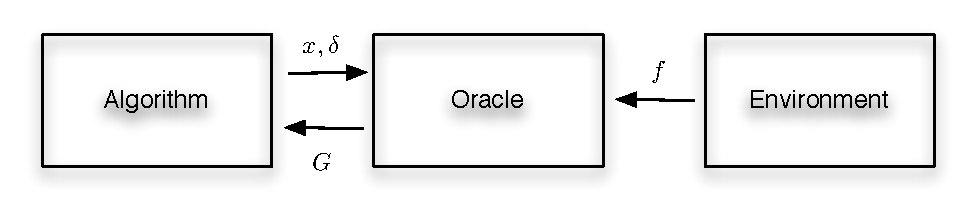
\includegraphics[width=\textwidth]{figs/oracle0}

	\ec	
	

\begin{enumerate}
\item Bias: $\norm{ \EE{G}  - \nabla f(x)  }_* \le c_1(\delta) $; and
\item Second moment: $\EE{\norm{ G  }_*^2} \le c_2(\delta)$.
\end{enumerate}

\bc
Controlled noise: $c_1(\delta) = C_1\delta^2$, $c_2(\delta) = C_2$.

Uncontrolled noise:  $c_1(\delta) = C_1\delta^2$, $c_2(\delta) = C_2 \delta^{-2}$.

\bigskip 
Polynomial oracle: $c_1(\delta) = C_1 \delta^p$, $c_2(\delta) = C_2 \delta^{-q}$, $p,q>0$.

\ec



}


\section{Results}
%%%%%%%%%%%%%%%%%%%%%%%%%%%%%%%%%%%%%%%%%%%%%%%%
\frame{
	\frametitle{Upper Bounds}
Algorithm: Mirror descent \citep{NeYu83}.

\begin{theorem}[\textit{\textbf{Upper bound}}]
Consider MD with a $(c_1,c_2)$, $(p,q)$ polynomial oracle, $\alpha$ SOC regularizer $\cR$.
Then:
\begin{align*}
\Delta_n(\F_{L,0},\mathrm{MD},c_1,c_2 ) &
= O( n^{- \frac{p}{2p+q} } )\\
% \le K_1\left(\dfrac{D {C_1^{\frac{q}{p}} C_2}}{ n}\right)^{\frac{p}{2p+q}},\\
\Delta_n(\F_{L,\mu},\mathrm{MD},c_1,c_2 ) &
= O( n^{- \frac{p}{p+q} } )\,.
%\le K_2\left(\dfrac{C_1^{\frac{q}{p}} C_2}{ n}\right)^{\frac{p}{p+q}},
\end{align*}
%where $D:=\sup_{x,y\in \cK} \DR(x,y)$, $K_1$ is a constant that depends on oracle parameters $p, q$ and strong convexity constant $\alpha$ of $\cal R$ and where $K_2$ is a constant that depends on $p, q, \alpha$ and $\mu$.
\end{theorem}
}

%%%%%%%%%%%%%%%%%%%%%%%%%%%%%%%%%%%%%%%%%%%%%%%%

\frame{
	\frametitle{Specific Rates}
Recall:
\begin{align*}
\Delta_n(\F_{L,0},\mathrm{MD},c_1,c_2 ) &
= O( n^{- \frac{p}{2p+q} } )\\
% \le K_1\left(\dfrac{D {C_1^{\frac{q}{p}} C_2}}{ n}\right)^{\frac{p}{2p+q}},\\
\Delta_n(\F_{L,\mu},\mathrm{MD},c_1,c_2 ) &
= O( n^{- \frac{p}{p+q} } )\,.
%\le K_2\left(\dfrac{C_1^{\frac{q}{p}} C_2}{ n}\right)^{\frac{p}{p+q}},
\end{align*}

\bigskip

$n^{-1/2}$ rate: $p/(2p+q)\ge 1/2$ vs. $p/(p+q)\ge 1/2$.\\
First holds iff $q=0$. Second holds iff $p\ge q$.\\

\bigskip

Uncontrolled noise: $p=q=2$. \\
For $\F_{L,\mu}$ we get $O(n^{-1/2})$ as \citet{HaLe14:SOC}.\\
For $\F_{L,0}$ we get $O(n^{-1/3})$ as \citet{saha2011improved}.

\bigskip

Controlled noise: $p=2$, $q=0$.\\
For $\F_{L,\mu}$ we get $O(1/n)$ as 
	\citet{Ne11:TR}	.\\
For $\F_{L,0}$ we get $O(n^{-1/2})$ as	
	\citet{duchi2015optimal}.

}
%%%%%%%%%%%%%%%%%%%%%%%%%%%%%%%%%%%%%%%%%%%%%%%%
\frame{
	\frametitle{Lower Bound}


\begin{theorem}[\textit{\textbf{Lower bound}}]
\label{thm:lb-convex}
$\cK\subset \R^d$ convex, closed, with  $\{+1,-1\}^d\subset \cK$, $n$ large enough.
For any algorithm $\mathrm{A}$ that observes $n$ random elements from a  $(p,q)$ polynomial oracle, we have
 \vspace*{-0.1in}
\begin{align*}
\Delta_n(\F_{L,0},\mathrm{A},c_1,c_2 ) &= \Omega( n^{-\frac{p}{2p+q}}),\\
\Delta_n(\F_{L,1},\mathrm{A},c_1,c_2 ) & = \Omega(  n^{-\frac{\alert{2}p}{2p+q}})\,.
\end{align*}
\end{theorem}
Compare with 
\begin{align*}
\Delta_n(\F_{L,0},\mathrm{MD},c_1,c_2 ) &
= O( n^{- \frac{p}{2p+q} } )\\
% \le K_1\left(\dfrac{D {C_1^{\frac{q}{p}} C_2}}{ n}\right)^{\frac{p}{2p+q}},\\
\Delta_n(\F_{L,1},\mathrm{MD},c_1,c_2 ) &
= O( n^{- \frac{p}{p+q} } )  = O(n^{-\frac{2p}{2p+\alert{2}q}})\,.
%\le K_2\left(\dfrac{C_1^{\frac{q}{p}} C_2}{ n}\right)^{\frac{p}{p+q}},
\end{align*}
(The lower bound for $\F_{L,0}$ is tight, for $\F_{L,1}$ it is weak.)
}
%%%%%%%%%%%%%%%%%%%%%%%%%%%%%%%%%%%%%%%%%%%%%%%%
\frame{
	\frametitle{A Corollary for Smooth Convex Optimization with Noisy Bandit Feedback}
\begin{Corollary}
To get the optimal $O(n^{-1/2})$ rate for $\F_{L,0}$  with uncontrolled noise,
one of the following must be done:
\begin{enumerate}
\item An oracle with $q=0$ (constant second moment bound) must be designed.
\item 
\sout{An algorithm that makes better use of the gradient estimates must be designed.}
\item Some extra properties of gradient estimates must be exploited beyond bias/variance.
\end{enumerate}
\end{Corollary}	
}
%%%%%%%%%%%%%%%%%%%%%%%%%%%%%%%%%%%%%%%%%%%%%%%%

\if0
\frame{
	\frametitle{}	
	\bc
	\begin{tabular}[t]{r|c|c|c|}
	 & Lower b. & Upper b. & Alg. \\
	 \hline
	 \hline
	 Convex & $\sqrt{d^2/n}$ & $\sqrt{d^2/n}$ & AAA \\
	 \hline
	 Smooth C. & $\sqrt{d^2/n}$ & $\sqrt{d^2/n}$ & AAA \\
	 \hline
	 Smooth + SOC & $\sqrt{d^2/n}$ & $\sqrt{d^2/n}$ & AAA \\
	 \hline
	\end{tabular}
	\ec
}
\fi

\if0
Convex opt 101:
Ellipsoid method
\fi
%%%%%%%%%%%%%%%%%%%%%%%%%%%%%%%%%%%%%%%%%%%%%%%%

%%%%%%%%%%%%%%%%%%%%%%%%%%%%%%%%%%%%%%%%%%%%%%%%



\begin{frame}
\begin{center}
\LARGE{Thanks! Questions?}
\end{center}
\end{frame}


%%%%%%%%%%%%%%%%%%%%%%%%%%%%%%%%%%%%%%%%%%%%%%%%%%%%%%%%%%%%%%%

%\begin{frame}
%\frametitle{}
%\end{frame}

%%%%%%%%%%%%%%%%%%%%%%%%%%%%%%%%%%%%%%%%%%%%%%%%%%%%%%%%%%%%%%%

\begin{frame}[allowframebreaks]
	\frametitle{References}
%        \begin{center}
%          Thanks!
%        \end{center}
	%\bibliographystyle{acm}
%	\begin{multicols}{2}
	\scriptsize 
	%\scriptsize\tiny
%	\bibliography{biblio,allbib,shortconfs,../thebib}
%	\bibliography{allbib,shortconfs,../thebib}
%\bibliography{allbib,shortconfs}
\bibliography{allbib,shortconfs,main}
%	\bibliography{../thebib}
%	\end{multicols}
\end{frame}


\end{document}
